% this is a template for papers or notes written in Chinese
\documentclass[a4paper]{report}

\makeatletter
\newcommand{\mytitle}{\@title}
\makeatother

\usepackage[
    fontset=none,%设置中文支持,并自定义字体
    zihao=5,%默认字号为五号
    heading=true,%允许后续自定义标题样式
    scheme=chinese,%自动将文档样式中文化,例如图标标题
    punct=quanjiao,%全角式标点符号
    space=auto,%中文后接换行不会添加空格,但是英文会添加空格,需要用%手动取消
    % linespread=1.3,%行距倍数是1.3
    autoindent=true,%自动缩进两个中文宽度
    ]{ctex}

\ctexset{
    today=small,%小写样式的日期
    contentsname={目录},
    % contentsname={\hspace{-\ccwd}目录},
    listfigurename={插图},
    listtablename={表格},
    figurename={图},
    tablename={表},
    abstractname={简{\quad}介},
    indexname={索引},
    appendixname={附录},
    bibname={参考文献},
    proofname={证明},
    % refname={参考文献},%只适用于beamer
    % algorithmname={算法},
    % continuation={(续)},%beamer续页的标识
    chapter={
        format+ = \Huge\heiti\raggedright,
        name = {,\num\textbf{.}\hspace{1ex}},
        number={\num\thechapter},
        nameformat={},
        numberformat={},
        aftername={},
        titleformat={},
        aftertitle={},
        runin=false,%对section级以下有用,标题是否和正文在同一段上
        beforeskip={3.5ex plus 1ex minus .2ex},%标题前垂直间距
        afterskip={2.3ex plus .2ex}%标题后垂直间距
    },
    section={
        format+ = \Large\heiti\raggedright,
        name = {,\num\textbf{.}\hspace{1ex}},
        number={\num\thesection},
        nameformat={},
        numberformat={},
        aftername={},
        titleformat={},
        aftertitle={},
        runin=false,%对section级以下有用,标题是否和正文在同一段上
        beforeskip={3.5ex plus 1ex minus .2ex},%标题前垂直间距
        afterskip={2.3ex plus .2ex}%标题后垂直间距
    },
    subsection={
        format+ = \large\heiti\raggedright,
        name = {,\num\textbf{.}\hspace{1ex}},
        number={\num\thesubsection},
        nameformat={},
        numberformat={},
        aftername={},
        titleformat={},
        aftertitle={},
        runin=false,%对section级以下有用,标题是否和正文在同一段上
        beforeskip={3.5ex plus 1ex minus .2ex},%标题前垂直间距
        afterskip={2.3ex plus .2ex}%标题后垂直间距
    },
    subsubsection={
        format+ = \normalsize\heiti\raggedright,
        name = {,\num\textbf{.}\hspace{1ex}},
        number={\num\thesubsubsection},
        nameformat={},
        numberformat={},
        aftername={},
        titleformat={},
        aftertitle={},
        runin=false,%对section级以下有用,标题是否和正文在同一段上
        beforeskip={3.5ex plus 1ex minus .2ex},%标题前垂直间距
        afterskip={2.3ex plus .2ex}%标题后垂直间距
    },
    }

\usepackage{amsfonts}
\usepackage{lmodern}%解决报错
% 中文默认字体: 思源宋体,粗体为思源宋体半粗体,斜体为方正楷体_GBK
\setCJKmainfont{Source Han Serif SC}[BoldFont={Source Han Serif SC Heavy}, ItalicFont=FZKai-Z03S]
% 中文无衬线字体:思源黑体,粗体为思源黑体粗体
\setCJKsansfont{Source Han Sans CN}[BoldFont={Source Han Sans CN Heavy}]
% 中文等宽字体:微软雅黑light
\setCJKmonofont{Microsoft YaHei}[ItalicFont={Microsoft YaHei Light}]

\newCJKfontfamily\songti{Source Han Serif SC}[BoldFont={Source Han Serif SC Heavy}]
\newCJKfontfamily\xbsong{Source Han Serif SC SemiBold} % 小标宋
\newCJKfontfamily\dbsong{Source Han Serif SC Bold} % 大标宋
\newCJKfontfamily\cusong{Source Han Serif SC Heavy} % 粗宋
\newCJKfontfamily\heiti{Source Han Sans CN}[BoldFont={Source Han Sans CN Heavy}]
\newCJKfontfamily\dahei{Source Han Sans CN Medium} % 大黑
\newCJKfontfamily\cuhei{Source Han Sans CN Heavy} % 粗黑
\newCJKfontfamily\fangsong{FZFangSong-Z02S}
\newCJKfontfamily\kaiti{FZKai-Z03S}[ItalicFont={Microsoft YaHei Light}]%这个斜体只是用于lstlisting环境中的中文注释
% \newCJKfontfamily\kaiti{FZKai-Z03S}[ItalicFont={FZZJ-LZXTFSJW}]%这个斜体只是用于lstlisting环境中的中文注释
\setsansfont{Arial}
\setmonofont{Consolas}%设置西文等宽字体
\newfontfamily\code{Consolas}
\newfontfamily\num{Arial}

\usepackage{geometry}%设置整体页面布局
\geometry{a4paper}
\geometry{left=2cm,right=2cm,top=2.54cm,bottom=2.54cm}%word常规页边距
% \geometry{left=1.27cm,right=1.27cm,top=1.27cm,bottom=1.27cm}%word窄页边距
\setlength{\headheight}{13pt}%避免warning


\usepackage{fancyhdr}%必须在geometry包之后使用
\fancyhf{}
\lhead{\sffamily\bfseries{范潇 2254298}}%可以使用thepage,CTEXthechapter,CTEXthesection
\chead{\sffamily\bfseries{课程设计作业Project5}}
\rhead{\sffamily\bfseries{- \thepage{} -}}
\renewcommand\headrulewidth{2pt}%设置眉头宽度
\pagestyle{fancy}


\usepackage{tikz}
\usepackage{graphicx}
\usepackage{longtable}
\usepackage{amssymb}
\newcommand*{\abs}[1]{\lvert #1 \rvert}
\setlength{\baselineskip}{18pt}
\usepackage{float}
\usepackage[ruled,algosection,lined,longend,fillcomment,linesnumbered,resetcount,titlenotnumbered]{algorithm2e}
%参数解释:带框,按section编码,有竖线,end前带if等关键词,注释占满整行,代码部分编号(不包括输入输出、注释),每个代码块重新编号,可以调用TitleOfAlgo来打印算法标题但不作为单独的算法编码
%附带algorithm,function,procedure环境,其中function,procedure环境下,设置caption时,必须带有(),
%()之前的字符会被视为宏,可以在接下来的部分用\名字()来调用,所以推荐辅助函数用function,其中的某些展开部分用procedure,描述算法整体使用algorithm
\DontPrintSemicolon
\SetAlCapSkip{2ex}
\SetSideCommentRight
\SetFillComment
\newcommand{\forcond}{$i=0$ \KwTo $n$}
\SetKw{macro}{text}%自定义关键词
\SetKwFunction{funcmacro}{text}%自定义函数名,实际上function环境是在定义宏的同时说明了其内容
\SetKwProg{procedmacro}{text}{begin text}{end text}%自定义步骤,和function类似,但是后面两个参数可以设置开始和结尾的标志,和if等环境一样
\SetKwData{datamacro}{text}%可以用于突出特殊的变量,例如数据结构
\SetKwFunction{FRecurs}{FnRecursive}
\SetKwProg{Fn}{Function}{begin}{end}
\usepackage{xcolor}%颜色支持
\definecolor{vscode_backgroundcolor}{rgb}{0.15, 0.2, 0.22}
\definecolor{vscode_localvariablecolor}{rgb}{0.93,1,0.89}
\definecolor{vscode_keywordcolor}{rgb}{0.57, 0.52, 1}
\definecolor{vscode_commentcolor}{rgb}{0.2, 0.34, 0.45}
\definecolor{vscode_stringcolor}{rgb}{0.76, 0.91, 0.55}
\definecolor{vscode_semicolomncolor}{rgb}{1,1,1}
\definecolor{vscode_headerfilecolor}{rgb}{0.93,1,0.89}
\definecolor{vscode_linenumbercolor}{rgb}{0.2, 0.34, 0.45}
\definecolor{vscode_numbercolor}{rgb}{0.96, 0.54, 0.42}
\definecolor{vscode_parametercolor}{rgb}{0.96, 0.54, 0.42}
\definecolor{vscode_operatorcolor}{rgb}{0.53, 0.85, 0.99}
\definecolor{vscode_callablecolor}{rgb}{0.36, 0.62, 0.96}
\definecolor{vscode_rulecolor}{rgb}{0.22, 0.28, 0.31}
\definecolor{vscode_classcolor}{rgb}{1, 0.8, 0.42}
\definecolor{vscode_selfcolor}{rgb}{0.97, 0.31, 0.43}

\usepackage{listings}%高亮代码块支持
\lstloadlanguages{Python}
\lstdefinestyle{MyPython}{
    extendedchars=false,
    numbers=left,
    firstnumber=auto,
    frame=leftline,
    backgroundcolor=\color{vscode_backgroundcolor},
    framerule=0.5ex,
    columns=fixed,
    language=Python,
    basicstyle=\ttfamily\color{vscode_localvariablecolor},
    % commentstyle=\color{vscode_commentcolor},
    keywordstyle=\color{vscode_keywordcolor},
    stringstyle=\color{vscode_stringcolor},
    morecomment=[l][\color{vscode_commentcolor}]{\#},
    morecomment=[s][\color{vscode_headerfilecolor}]{"""}{"""},
    numberstyle=\code\color{vscode_linenumbercolor},
    morekeywords={
        None,
        True,
        yield,
        False,
    },
    alsoletter={
        =+-*<>^&
        % ;0123456789
        % 0,1,2,3,4,5,6,7,8,9
    },%把;设置为可以识别的letter,也可以使用otherkeywords,但是无法将其和其他keywords区分开来
    emph={=,+,-,*,>,<,<<,>>,^,+=,&},emphstyle=\color{vscode_operatorcolor},
    % alsoletter={!,\%,&,*,-,+,=,/,<,>},
    emph={[2]%一些全局的函数和可调用对象
    namedtuple,
    list2tuple,
    list,
    tuple, 
    generalGraphSearch,
    float,
    isinstance,
    Property,
    PriorityQueue,
    getSuccessors,
    getStartState,
    isGoalState,
    push,
    pop,
    isEmpty,
    get_solution,
    keys,
    cnt,
    next,
    dfsPriority,
    bfsPriority,
    ucsPriority,
    AStarPriority,
    append,
    aStarSearch,
    depthFirstSearch,
    breadthFirstSearch,
    uniformCostSearch,
    len,
    index,
    Successors,
    int,
    directionToVector,
    greedy,
    manhattanDistance,
    remove,
    cornersHeuristic,
    enumerate,
    foodHeuristic,
    max,
    range,
    asList,
    findPathToClosestDot,
    getPacmanPosition,
    getFood,
    getWalls,
    AnyFoodSearchProblem,
    evaluationFunction,
    generatePacmanSuccessor,
    getGhostStates,
    float,
    len,
    maximize,
    minimize,
    getLegalActions,
    evaluationFunction,
    generateSuccessor,
    getNumAgents,
    randomMove,
    run,
    train,
    get,
    prediction,
    iterate,
    once,
    as,
    scalar,
    DotProduct,
    update,
    Parameter,
    AddBias,
    Linear,
    ReLU,
    SquareLoss,
    gradients,
    init,
    mid,
    log,
    SoftmaxLoss
    },emphstyle={[2]\color{vscode_callablecolor}},
    emph={[5]
    self},emphstyle={[5]\color{vscode_selfcolor}},
    % emphstyle={[3]\color{vscode_parametercolor}}
     % emph={[3]0,1,2,3,4,5,6,7,8,9},emphstyle={[3]\color{yellow}},
    tabsize=4,
    rulecolor=\color{vscode_rulecolor},
    breaklines=true,
}
\lstset{
    style=MyPython,
}
% \usepackage{xcolor}%颜色支持
\definecolor{vscode_backgroundcolor}{rgb}{0,0.14,0.32}
\definecolor{vscode_localvariablecolor}{rgb}{0.94,0.62,0.64}
\definecolor{vscode_keywordcolor}{rgb}{0.92,0.73,1}
\definecolor{vscode_commentcolor}{rgb}{0.55,0.64,0.79}
\definecolor{vscode_stringcolor}{rgb}{0.05,0.95,0.86}
\definecolor{vscode_semicolomncolor}{rgb}{1,1,1}
\definecolor{vscode_headerfilecolor}{rgb}{0.82,0.95,0.65}
\definecolor{vscode_linenumbercolor}{rgb}{0.52,0.52,0.52}
\definecolor{vscode_numbercolor}{rgb}{1,0.77.0.56}
\definecolor{vscode_operatorcolor}{rgb}{0.6,1,1}
\definecolor{vscode_functioncolor}{rgb}{0.22,0.65,0.96}
\definecolor{vscode_rulecolor}{rgb}{0.17,0.46,0.65}

\usepackage{amsmath}%必须在amsthm之前
\usepackage{amsthm}%提供证明,定理等环境

\theoremstyle{plain}
\newtheorem{thm}{Theorem}[section]
\newtheorem{lmm}{Lemma}[section]
\newtheorem{cor}{Corollary}[section]
\newtheorem{prop}{Proposition}[section]
\newtheorem{conj}{Conjecture}[section]

\theoremstyle{definition}
\newtheorem{definition}{Definition}[section]
\newtheorem*{cond}{Condition}
\newtheorem{eg}{Example}[section]
\newtheorem{exer}{Exercise}[section]
\newtheorem*{property}{Property}

\theoremstyle{remark}
\newtheorem*{rmk}{Remark}


\usepackage[strict]{changepage}
\usepackage{framed}%色块支持
\definecolor{formalshade}{rgb}{0.95,0.95,1} % 文本框颜色
% ------------------******-------------------
% 注意行末需要把空格注释掉,不然画出来的方框会有空白竖线

\definecolor{theorem_bar_color}{RGB}{183, 28, 28}
\definecolor{theorem_box_color}{RGB}{255, 235, 238}
\newenvironment{mythm}[1][]{%
\def\FrameCommand{%
\hspace{1pt}%
{\color{theorem_bar_color}\vrule width 2pt}%
{\color{theorem_box_color}\vrule width 4pt}%
\colorbox{theorem_box_color}%
}%
\MakeFramed{\advance\hsize-\width\FrameRestore}%
\noindent\hspace{-4.55pt}% disable indenting first paragraph
\begin{adjustwidth}{}{7pt}%
\begin{thm}[#1]
    \quad\par
}
{%
\end{thm}
\vspace{2pt}\end{adjustwidth}\endMakeFramed%
}

\definecolor{corollary_bar_color}{RGB}{26, 35, 126}
\definecolor{corollary_box_color}{RGB}{232, 234, 246}
\newenvironment{mycor}[1][]{%
\def\FrameCommand{%
\hspace{1pt}%
{\color{corollary_bar_color}\vrule width 2pt}%
{\color{corollary_box_color}\vrule width 4pt}%
\colorbox{corollary_box_color}%
}%
\MakeFramed{\advance\hsize-\width\FrameRestore}%
\noindent\hspace{-4.55pt}% disable indenting first paragraph
\begin{adjustwidth}{}{7pt}%
\begin{cor}[#1]
    \quad\par
}
{%
\end{cor}
\vspace{2pt}\end{adjustwidth}\endMakeFramed%
}

\definecolor{lemma_bar_color}{RGB}{74, 20, 140}
\definecolor{lemma_box_color}{RGB}{243, 229, 245}
\newenvironment{mylmm}[1][]{%
\def\FrameCommand{%
\hspace{1pt}%
{\color{lemma_bar_color}\vrule width 2pt}%
{\color{lemma_box_color}\vrule width 4pt}%
\colorbox{lemma_box_color}%
}%
\MakeFramed{\advance\hsize-\width\FrameRestore}%
\noindent\hspace{-4.55pt}% disable indenting first paragraph
\begin{adjustwidth}{}{7pt}%
\begin{lmm}[#1]
    \quad\par
}
{%
\end{lmm}
\vspace{2pt}\end{adjustwidth}\endMakeFramed%
}

\definecolor{proposition_bar_color}{RGB}{1, 87, 155}
\definecolor{proposition_box_color}{RGB}{225, 245, 254}
\newenvironment{myprop}[1][]{%
\def\FrameCommand{%
\hspace{1pt}%
{\color{proposition_bar_color}\vrule width 2pt}%
{\color{proposition_box_color}\vrule width 4pt}%
\colorbox{proposition_box_color}%
}%
\MakeFramed{\advance\hsize-\width\FrameRestore}%
\noindent\hspace{-4.55pt}% disable indenting first paragraph
\begin{adjustwidth}{}{7pt}%
\begin{prop}[#1]
    \quad\par
}
{%
\end{prop}
\vspace{2pt}\end{adjustwidth}\endMakeFramed%
}

\definecolor{definition_bar_color}{RGB}{0, 77, 64}
\definecolor{definition_box_color}{RGB}{224, 242, 241}
\newenvironment{mydef}[1][]{%
\def\FrameCommand{%
\hspace{1pt}%
{\color{definition_bar_color}\vrule width 2pt}%
{\color{definition_box_color}\vrule width 4pt}%
\colorbox{definition_box_color}%
}%
\MakeFramed{\advance\hsize-\width\FrameRestore}%
\noindent\hspace{-4.55pt}% disable indenting first paragraph
\begin{adjustwidth}{}{7pt}%
\begin{definition}[#1]
    \quad\par
}
{%
\end{definition}
\vspace{2pt}\end{adjustwidth}\endMakeFramed%
}

\definecolor{remark_bar_color}{RGB}{245, 127, 23}
\definecolor{remark_box_color}{RGB}{255, 253, 231}
\newenvironment{myrmk}[1][]{%
\def\FrameCommand{%
\hspace{1pt}%
{\color{remark_bar_color}\vrule width 2pt}%
{\color{remark_box_color}\vrule width 4pt}%
\colorbox{remark_box_color}%
}%
\MakeFramed{\advance\hsize-\width\FrameRestore}%
\noindent\hspace{-4.55pt}% disable indenting first paragraph
\begin{adjustwidth}{}{7pt}%
\begin{rmk}[#1]
    \quad\par
}
{%
\end{rmk}
\vspace{2pt}\end{adjustwidth}\endMakeFramed%
}

\definecolor{property_bar_color}{RGB}{62, 39, 35}
\definecolor{property_box_color}{RGB}{239, 235, 233}
\newenvironment{myproperty}[1][]{%
\def\FrameCommand{%
\hspace{1pt}%
{\color{property_bar_color}\vrule width 2pt}%
{\color{property_box_color}\vrule width 4pt}%
\colorbox{property_box_color}%
}%
\MakeFramed{\advance\hsize-\width\FrameRestore}%
\noindent\hspace{-4.55pt}% disable indenting first paragraph
\begin{adjustwidth}{}{7pt}%
\begin{property}[#1]
    \quad\par
}
{%
\end{property}
\vspace{2pt}\end{adjustwidth}\endMakeFramed%
}

\author{\Large{范潇\quad2254298}}
\title{\sffamily\Huge\bfseries{人工智能课程Project1}}
\date{\Large{\today}}
\begin{document}
\begin{titlepage}
    \heiti
    \vspace*{64pt}
    \begin{center}
        
\includegraphics{./pic/tongji-logo-purple.pdf}
        % \fontsize{72pt}{0} 南华大学\\

        \vspace*{36pt}
        \fontsize{48pt}{0}{实\quad 验\quad 报\quad 告}\\
        \vspace*{48pt}
        \LARGE(2023\~{}2024学年第二学期)\\
        \vspace*{48pt}
    
        \LARGE 课程名称\ \ \underline{\makebox[200pt]{人工智能课程设计}}\\
        \LARGE 实验名称\ \ \underline{\makebox[200pt]{课程设计作业Project1}}\\
        \vspace*{36pt}
    
        \Large 姓名\ \ \underline{\makebox[108pt]{范潇}}\ \ 学号\ \ \underline{\makebox[108pt]{2254298}}\\
        % \Large 学院\ \ \underline{\makebox[108pt]{}}\ \ 班级\ \ \underline{\makebox[108pt]{}}\\
        % \Large 地点\ \ \underline{\makebox[108pt]{}}\ \ 教师\ \ \underline{\makebox[108pt]{}}\\
    \end{center}
\end{titlepage}
% \maketitle
% \thispagestyle{fancy}%用于单独设置某页的样式,此处用于设置标题页的格式
\chapter{项目概述}
\section{主要内容与目标}
本次项目的主要内容为搜索算法。具体目标是实现算法使得吃豆人能够在迷宫中达到特定的位置,同时高效地收集食物。因此,本项目中的状态只需包含当前位置,
如果要求需要收集多处食物,则还需要包含存储相应记录的数组。

本项目的八个问题可以分为三部分。

第一部分的任务是搜索问题是到达迷宫中指定的位置,要求分别使用DFS,BFS,UCS以及$A^*$算法实现。在该部分中,用于测试的迷宫有tinyMaze,mediumMaze,bigMaze,openMaze,
前三个迷宫中只有一处食物,即目标状态。openMaze的特点在于迷宫的墙壁较为稀疏。

第二部分的任务是对于指定搜索任务进行形式化,并构造相应的启发式函数。在该部分中,搜索任务的目标是让吃豆人到达迷宫的四个角落。

第三部分的任务围绕“收集迷宫中的所有食物”这一搜索问题展开,要求设计启发式函数以及不追求最优解的算法。
\section{已有代码}
下面对已有代码中与本项目的具体实现相关的代码进行分析。
\subsection{util.py}
该文件中提供了多种可能需要用到的数据结构,并且如果需要使用,不能用Python自带库代替,因为可能会影响自动评分程序。
\begin{enumerate}
\item Stack:有push,pop,isEmpty方法,分别用于进行压栈、出栈以及判断栈是否为空的操作。
\item Queue:有push,pop,isEmpty方法,分别用于入队、出队以及判断队列是否为空的操作。
\item PriorityQueue:有push,pop,isEmpty,update方法,分别用于入队、出队、判断队列是否为空以及更新元素有限度的操作。优先弹出优先级低的元素。
\item PriorityQueueWithFunction:是PriorityQueue的子类,支持指定一个函数priorityFunction用于从存储元素中提取优先级。
\end{enumerate}
这些数据结构的底层都是用列表实现的。

同时还提供了用于计算曼哈顿距离的函数manhattanDistance。
\subsection{search.py}
该文件用于存储各种搜索算法的实现,同时包含了抽象类SearchProblem。

SearchProblem类有以下方法:
\begin{enumerate}
    \item getStartState(self):返回初始状态
    \item isGoalState(self,state):对所给状态进行目标测试
    \item getSuccessors(self,state):返回三元组(successor,action,stepCost),其中successor为所给状态的后继,action为对应的状态,stepCost为action对应的代价
    \item getCostOfActions(self,actions):输入为一系列合法动作,返回对应的代价总和。
\end{enumerate}
同时,该文件还给出了一个样例:tinyMazeSearch(problem)。从中可以了解到需要自行实现的算法返回的解序列的形式是一个列表,元素为game库中导入的Directions类。
\subsection{searchAgents.py}
该文件中存储的是关于智能体以及搜索问题相关的代码,并不包含搜索算法的实现。

PositionSearchProblem类是SearchProblem类的子类,用于存储状态空间中只包含位置的搜索问题。具体细节有:
\begin{enumerate}
\item 状态用二元元组实现
\item 当行动非法,即产生“穿墙”行为时,代价返回999999
\end{enumerate}
从该类的代码中可以了解到初始化一个问题的基本步骤为:
\begin{enumerate}
    \item 初始化墙
    \item 获取吃豆人初始位置
    \item 设置起始状态
    \item 设置目标测试
    \item 设置损失函数
\end{enumerate}
同时,该文件还提供了函数mazeDistance。该函数通过广度优先搜索来获取迷宫内两点之间的最短路径长度。
\chapter{Question1}
\section{问题概述}
%
%%对问题的直观描述
%
本问题要求改进已有的基于反射的智能体。这里需要考虑有多个幽灵的场景,默认情况下幽灵的行动是随机的,最后评分的依据首先是能够确保吃豆人不被幽灵击败并收集到所有的食物,
然后是分数尽可能地高。


%
%对项目已有代码的阅读和理解
%

%
%解决问题的思路和想法
%

\section{算法设计}
已有代码中实现的智能体选择下一个行为的唯一依据是下一个状态的得分。这不仅导致吃豆人收集所有
食物的效率大大降低——当四周没有食物时,很有可能会来回兜圈子,更重要的是,这几乎没有考虑幽灵对于吃豆人的影响——吃豆人可能会移动到幽灵的相邻位置,这导致
吃豆人暴露在被幽灵吃掉的风险之中,而这并不能体现在下一个状态的得分之中,因为这需要涉及到再下一个状态。

为此,应该充分利用幽灵的位置信息和剩余食物的位置信息,使得确保吃豆人不会被幽灵击败的前提下尽可能高效地收集所有食物。
为了保证吃豆人的安全,我们只需要确保下一个状态和幽灵的曼哈顿距离不小于等于1即可。

在确保没有被幽灵击败的前提下,我优先让吃豆人选择直接收集到食物的动作,如果没有,则以到最近的食物的曼哈顿距离的相反数为评估函数,即采用贪心的策略,让吃豆人缩短其到最近的食物的距离。
%
%用自己的语言描述解决问题所使用的算法的原理及功能,设计思路和算法流程图
%
\section{算法实现}
%
%在算法原理的基础上,结合代码,讲述算法的实现细节、核心函数、模块输入输出,数据结构定义等内容
%
\begin{lstlisting}[emph={[3]currentGameState,action},emphstyle={[3]\color{vscode_parametercolor}},emph={[4]GameState},emphstyle={[4]\color{vscode_classcolor}}]
def evaluationFunction(self, currentGameState: GameState, action):
    successorGameState = currentGameState.generatePacmanSuccessor(action)
    newPos = successorGameState.getPacmanPosition()
    newFood = successorGameState.getFood()
    newGhostStates = successorGameState.getGhostStates()
    newScaredTimes = [ghostState.scaredTimer for ghostState in newGhostStates]

    if action == 'Stop':  # 不允许停止
        return -float('inf')
    newGhostPos = [ghostState.configuration.pos for ghostState in newGhostStates]
    # 只有当不进入无敌状态时才要考虑和幽灵之间的距离
    if sum(newScaredTimes) == 0 and min([manhattanDistance(ghostPos, newPos) for ghostPos in newGhostPos]) <= 1:
        return -float('inf')
    foods = newFood.asList()
    # 没有食物,即该步使得游戏胜利
    if not foods:
        return float('inf')
    score = -min([manhattanDistance(food, newPos) for food in foods]) - 100000 * len(foods)
    return score
\end{lstlisting}
这里要求吃豆人永远不停止不动,但实际上,在特别极端的情况下,例如吃豆人位于角落,幽灵处于它的紧邻的对角位置时,静止不动以观察幽灵的下一步才是正确的。
实现时,我用惩罚项-100000*len(foods)来体现出收集食物的优先性。值得注意的是,如果某个动作使得吃豆人收集到了一个食物,那么在进入该函数时,
该食物已经从食物列表中移除出来了,如果仅仅依据到食物列表中各个食物的曼哈顿距离的最小值,是无法判断出这一步究竟是否能够收集到食物的。
\section{实验结果}
%
%对试验结果进行详细展示,对每个问题展示测试截图,对于测试用例进行描述说明,对于为通过测试的用例结合自己的算法进行分析,可以结合调试过程进行分析
%
我成功获得了本问题的所有分数。
\begin{figure}[htbp]
    \centering
    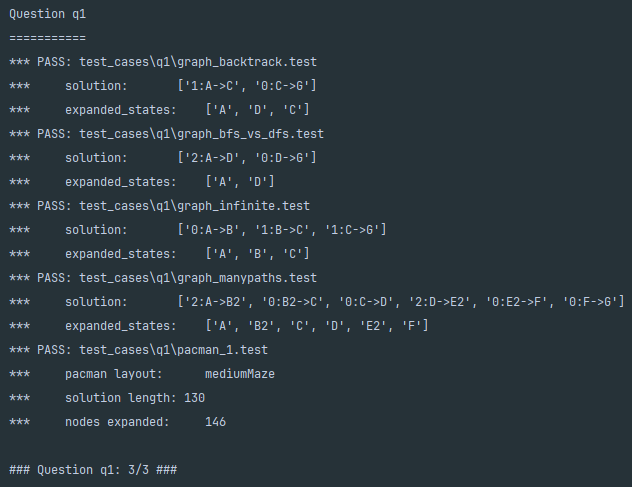
\includegraphics[scale = 0.7]{pic/q1.png}
    \caption{Question1实验结果}\label{q1}
\end{figure}

本问题的测试方式如图\ref{q1test}所示。该地图中没有墙壁,且只有一个随机移动的幽灵。通过该测试可以说明我所实现的算法能够指导吃豆人高效地收集所有的食物,
同时避免被幽灵击败。同时,我还额外对于有两个幽灵、有墙壁的中等迷宫场景进行了测试,如图\ref{q1ext},在连续两次测试中都成功收集所有的食物,结果如图\ref{q1extrst}所示。

\begin{figure}[htbp]
    \centering
    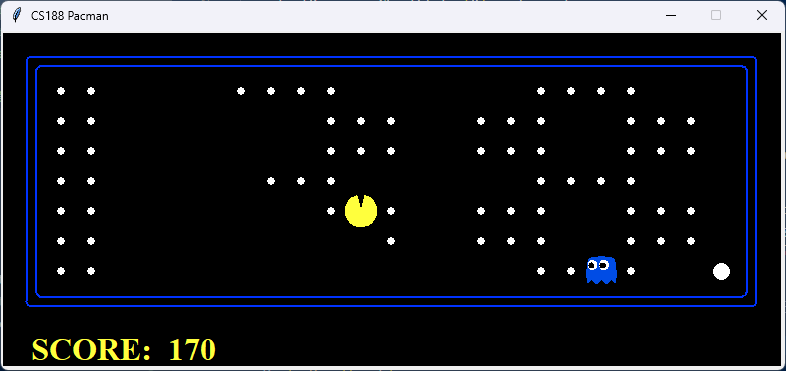
\includegraphics[scale = 0.5]{pic/q1test.png}
    \caption{Question1测试样例}\label{q1test}
\end{figure}
\begin{figure}[htbp]
    \centering
    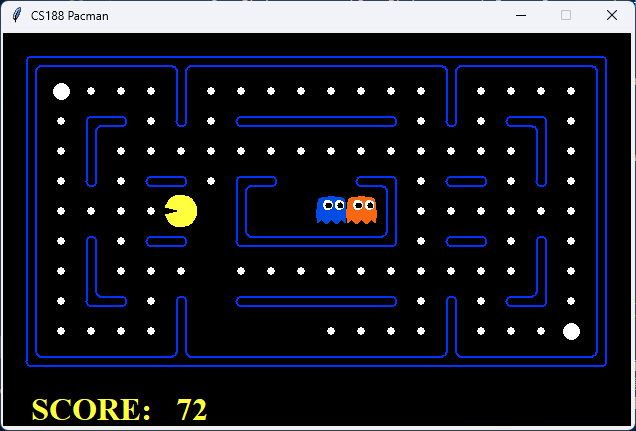
\includegraphics[scale = 0.5]{pic/q1ext.png}
    \caption{中等迷宫测试场景}\label{q1ext}
\end{figure}
\begin{figure}[htbp]
    \centering
    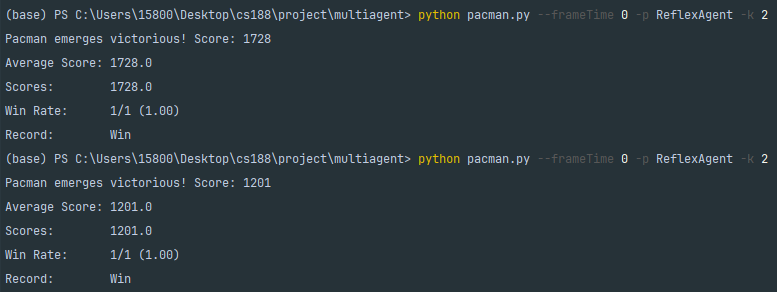
\includegraphics[scale = 0.8]{pic/q1extrst.png}
    \caption{中等迷宫测试结果}\label{q1extrst}
\end{figure}
%
%实验中遇到的问题及解决方案,收获和思考:对算法的理解、优缺点的评价、算法的适用场景
%

\chapter{Question2}
\section{问题概述}
%
%%对问题的直观描述
%
本问题要求实现Minimax算法,其中正方只有一个智能体,即吃豆人,但是反方,即幽灵,可能有多个。
%
%对项目已有代码的阅读和理解
%
%
%解决问题的思路和想法
%
\section{算法设计}
%
%用自己的语言描述解决问题所使用的算法的原理及功能,设计思路和算法流程图
%
由于可能有多个反方,所以在博弈树中,对应着正方的每一层下方都紧接着$n$层反方的结点,其中$n$为反方的个数。同时,
题目明确要求当层数到达给定值后,便使用评估函数,其中,“一层”对应着一轮游戏,即吃豆人和所有的幽灵都轮流各走了一步。

\begin{algorithm}[h]
    \SetKw{maximize}{maximize} 
    dummy,action = \maximize(gameState,1)\tcp*[h]{这里无需返回的分数}\;
    \Return{action}
    \caption{Minimax(gameState)}
\end{algorithm}

\begin{procedure}[h]
    \KwOut{bestScore,bestAction}
    \SetKw{in}{in}
    \SetKw{minimize}{minimize}
    \tcp*[h]{给定状态和对应深度,返回从当前状态出发所能达到的最佳分数和对应的动作}\;
    actions = gameState.getLegalActions()\;
    ghostNum = gameState.getNumAgent - 1\;
    \If{depth > depthLimit or actions == None}
    {\Return{evaluationFunction(gameState),None}\tcp*[h]{无法继续行动,直接返回当前状态的分数}}
    bestScore = $-\infty$\;
    bestAction = None\;
    \ForEach{action \in actions}
    {
        next = gameState.generateSuccessor(gameState,action)\tcp*[h]{获取下一个状态}\;
        score,dummy = \minimize(next,1,ghostNum,depth)\tcp*[h]{这里并不需要返回的动作}\;
        \If{score > bestScore}
        {
            bestAction = action\;
            bestScore = score\;
        }
    }
    \Return{bestScore,bestAction}
    \caption{maximize(gameState,depth)}
\end{procedure}

\begin{procedure}[h]
    \KwOut{bestScore,bestAction}
    \SetKw{in}{in}
    \SetKw{minimize}{minimize}
    \tcp*[h]{给定状态和对应深度,返回从当前状态出发所能达到的最佳分数和对应的动作}\;
    actions = gameState.getLegalActions()\;
    \If{depth > depthLimit or actions == None}
    {\Return{evaluationFunction(gameState),None}\tcp*[h]{无法继续行动,直接返回当前状态的分数}}
    bestScore = $\infty$\;
    bestAction = None\;
    \ForEach{action \in actions}
    {
        next = gameState.generateSuccessor(gameState,action)\tcp*[h]{获取下一个状态}\;
        \eIf{ghostNo == ghostNum}
        {
            score,dummy = \maximize(next,depth+1)\tcp*[h]{当前智能体是最后一个幽灵,下一层为吃豆人}
        }
        {
        score,dummy = \minimize(next,ghostNo+1,ghostNum,depth)\tcp*[h]{这里并不需要返回的动作}
        }
        \If(\tcp*[h]{对于幽灵而言,目标是让吃豆人的分数尽可能的低}){score < bestScore}
        {
            bestAction = action\;
            bestScore = score\;
        }
    }
    \Return{bestScore,bestAction}
    \caption{minimize(gameState,ghostNo,ghostNum,depth)}
\end{procedure}

Minimax算法的核心是递归,并且使用的前提是博弈双方是理性的。maximize,minimize函数分别用于给出正反方的下一步以及对应的最优解的分数。
当无法继续行动时,当前状态是唯一可行的状态,自然是最优解。如果可以正方行动,那么在行动前,由于反方是理性的,正方需要枚举所有可能的行为,通过调用minimize
推算反方的反应和最终的结果,并最终选取出最佳的下一步。反方亦然。特别之处在于有多位反方,由于算法中的score统一是指正方的分数,所以无论是调用minimize的反方,
还是最后一位调用maximize的反方,其选取下一步的依据都是让score最小。

如果不在指定的深度调用评估函数,那么Minimax算法可能会产生无穷深的博弈树,这是不可接受的。
\section{算法实现}
\begin{lstlisting}[emph={[3]currentGameState,gameState,depth},emphstyle={[3]\color{vscode_parametercolor}},emph={[4]GameState,MinimaxAgent},emphstyle={[4]\color{vscode_classcolor}}]
class MinimaxAgent(MultiAgentSearchAgent):
    def maximize(self, gameState: GameState, depth: int):
        actions = gameState.getLegalActions(0)
        if depth > self.depth or not actions:
            return self.evaluationFunction(gameState), None
        bestScore = -float('inf')
        bestAction = None
        for action in actions:
            next = gameState.generateSuccessor(0, action)
            score, _ = self.minimize(next, 1, gameState.getNumAgents() - 1, depth)
            if score > bestScore:
                bestAction = action
                bestScore = score
        return bestScore, bestAction

    def minimize(self, gameState: GameState, ghostNo: int, ghostNum: int, depth: int):
        actions = gameState.getLegalActions(ghostNo)
        if not actions:
            return self.evaluationFunction(gameState), None
        bestScore = float('inf')
        bestAction = None
        for action in actions:
            next = gameState.generateSuccessor(ghostNo, action)
            if ghostNo == ghostNum:
                score, _ = self.maximize(next, depth + 1)
            else:
                score, _ = self.minimize(next, ghostNo + 1, ghostNum, depth)
            if score < bestScore:
                bestScore = score
                bestAction = action
        return bestScore, bestAction

    def getAction(self, gameState: GameState):
        return self.maximize(gameState, 1)[1]
\end{lstlisting}
\section{实验结果}
%
%对试验结果进行详细展示,对每个问题展示测试截图,对于测试用例进行描述说明,对于为通过测试的用例结合自己的算法进行分析,可以结合调试过程进行分析
%
我成功获得了本问题的所有分数,图\ref{q2}为实验结果。测试用例分为以下几类:
\begin{enumerate}
    \item eval-function-lose-states,eval-function-win-states:测试内容为一颗高度为2的博弈树,目的在于测试算法是否判断当前状态为胜负已定,并调用评估函数
    \item lecture-6-tree,small-tree,minmax:测试内容为Minimax的基本功能
    \item vary-depth:在minmax测试的基础上,对深度的限制进行调整,以测试算法是否正确处理该情况
    \item x-ghost-xlevel:测试了多位反方和多层深度限制的情况
    \item tied-root:测试了算法是否正确处理得分相同的情况
    \item check-depth-x-ghost:重点测试了算法是否正确处理深度限制
    \item pacman-game:在小型迷宫中使用Minimax算法进行实战
\end{enumerate}
\begin{figure}[H]
    \centering
    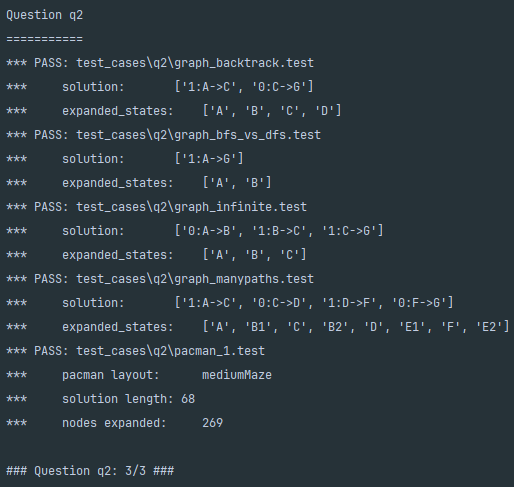
\includegraphics[scale = 0.8]{pic/q2.png}
    \caption{Question2实验结果}\label{q2}
\end{figure}
%
%在算法原理的基础上,结合代码,讲述算法的实现细节、和兴函数、模块输入输出,数据结构定义等内容
%
%
%对试验结果进行详细展示,对每个问题展示测试截图,对于测试用例进行描述说明,对于为通过测试的用例结合自己的算法进行分析,可以结合调试过程进行分析
%
%实验中遇到的问题及解决方案,收获和思考:对算法的理解、优缺点的评价、算法的适用场景
%

\chapter{Question3}
\section{问题概述}
%
%%对问题的直观描述
%
本问题要求利用神经网络进行数字分类。

%
%对项目已有代码的阅读和理解
%

%
%解决问题的思路和想法
%

\section{算法设计}
%
%用自己的语言描述解决问题所使用的算法的原理及功能,设计思路和算法流程图
%
所用的神经网络架构与上一题一样,唯一的区别在于特征向量维数从1变为了$28\times28$,输出向量维数由1变为了10,同时判断训练是否结束
的依据变为了由在验证集上得到的准确率。
\section{算法实现}
%
%在算法原理的基础上,结合代码,讲述算法的实现细节、核心函数、模块输入输出,数据结构定义等内容
%
%
\begin{lstlisting}[emph={[3]dataset,x,y},emphstyle={[3]\color{vscode_parametercolor}},emph={[4]DigitClassificationModel,RegressionModel,GameState,MinimaxAgent,AlphaBetaAgent},emphstyle={[4]\color{vscode_classcolor}}]
class DigitClassificationModel(object):
    def __init__(self):
        self.layer_size = 512
        self.feature_num = 28*28
        self.output_num = 10
        self.learning_rate = 0.5
        self.batch_size = 200
        self.threshold = 0.98
        self.w1 = nn.Parameter(self.feature_num,self.layer_size)
        self.b1 = nn.Parameter(1,self.layer_size)
        self.w2 = nn.Parameter(self.layer_size,self.output_num)
        self.b2 = nn.Parameter(1,self.output_num)
        self.W = [self.w1,self.b1,self.w2,self.b2]

    def run(self, x):
        return nn.AddBias( nn.Linear( nn.ReLU( nn.AddBias( nn.Linear(x,self.w1),self.b1)),self.w2),self.b2)

    def get_loss(self, x, y):
        return nn.SoftmaxLoss(self.run(x),y)

    def train(self, dataset):
        for x,y in dataset.iterate_forever(self.batch_size):
            gradients = nn.gradients(self.get_loss(x,y),self.W)
            for i,w in enumerate(self.W):
                w.update(gradients[i],-self.learning_rate)
            if dataset.get_validation_accuracy() >= self.threshold:
                break
\end{lstlisting}
\section{实验结果}
我成功获得了本问题的所有分数。本问的评分依据便是训练好的神经网络在测试集上得到的准确率。
\begin{figure}[htbp]
    \centering
    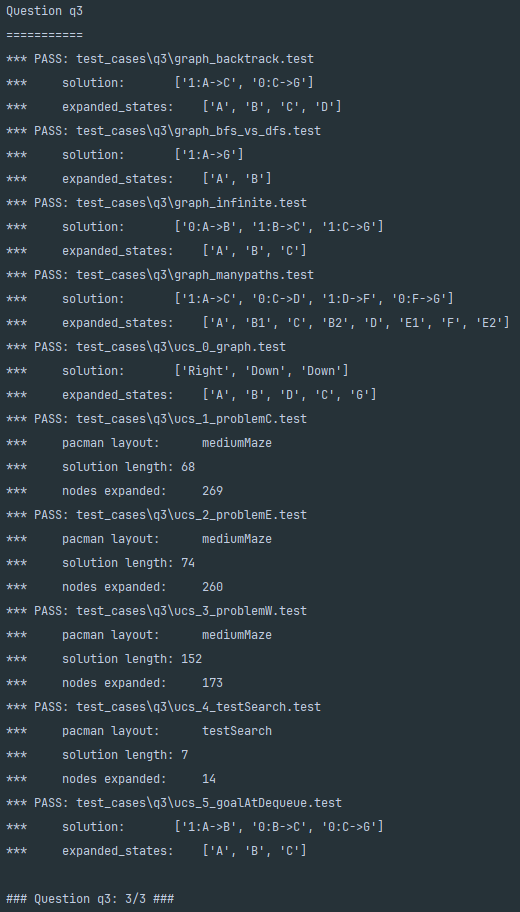
\includegraphics{pic/q3.png}
    \caption{Question3实验结果}\label{q3}
\end{figure}
%
%实验中遇到的问题及解决方案,收获和思考:对算法的理解、优缺点的评价、算法的适用场景
%

\chapter{总结与分析}
%
%实验中遇到的问题及解决方案,收获和思考:对算法的理解、优缺点的评价、算法的适用场景
%
通过本次实验,我深刻体会到了机器学习以及神经网络的强大之处。

在实验过程中,我主要遇到了三个问题。

其一,在完成问题二的过程中,起初,我并没有在线性层中增加偏置值。从可视化的结果中可以看出,由模型得到的曲线只是两段从原点引出的射线。而当我
添加了偏置值后,由模型得到的曲线很快便接近正弦函数的形态。

其二,在完成神经网络的相关题目时,我发现如果编程过程中把有关问题的参数以硬编码的方式保留下来,将会大大降低代码的可移植性和可读性,
同时,还不便于推导所需矩阵的形状。为此,我重构了自己的代码,将参数在\_\_init\_\_函数中便初始化,而非以魔数的形式在后续的训练过程中使用。
这使得我在完成第三题时,可以直接使用第二题的代码,只需修改输入输出的相关参数即可。

其三,在完成第四题的过程中,我体会到了超参数的重要性。一开始,我沿用前两题的两层线性层的神经网络架构,但是尝试了如0.5,0.1,0.01等多个学习率
后,结果都是在达到所需的准确率之前便产生了梯度消失或梯度爆炸的现象。为此,我将神经网络架构调整为了总共有三层线性层的架构。在
相同的其他超参数的条件下,新得到的神经网络便能成功达到所需的准确率。

在训练神经网络的过程中,我也观察到神经网络的准确率不一定时随着训练时间递增的,会有一定的波动存在,为此,在最后一题中,我设定停止训练的准确率阈值为87\%,
以增加在测试集上达到81\%准确率的概率。当然这样做的代价便是训练时间会增长一倍左右。我最终使用的神经网络能够在训练了60个epoch后达到80\%左右的准确率,
训练了100个epoch后能达到85\%左右的准确率,而为了达到87\%的准确率,需要训练180个epoch左右,这需要20分钟左右的时间。
\end{document}